The Hazard Modeller's Toolkit (or ``openquake.hmtk'') is a Python library of functions originally written by scientists at the GEM Model Facility, and now maintained by the GEM Foundation Secretariat. The HMTK is intended to provide 
scientists and engineers with the tools to help create the seismogenic 
input models that go into the OpenQuake hazard engine. The process of 
developing a hazard model is a complex and often challenging 
one, and while many aspects of the practice are relatively common, the 
choice of certain methods or tools for undertaking each step can be a 
matter of judgement. The intention of this software is to provide 
scientists and engineers with the means to apply many of the most 
commonly used algorithms for preparing seismogenic source models 
using seismicitiy and geological data. 

This manual is Version 2.0 of the HMTK tutorial. The major differences in the toolkit and the tutorial compared to the original release are i) the HMTK is now contained in the OpenQuake Engine, and does not require any separate installation, ii) the OpenQuake $hazardlib$ source classes have been adopted in order to ensure full compatibility and consistency between the two libraries, and iii) the plotting functions that produce maps now use Generic Mapping Tools (GMT) and Python scripts housed in the OpenQuake Model Building Toolkit. 


\section{The Development Process}

The Hazard Modeller's Toolkit is developed by GEM, and has occurred in several different stages. The present version makes the modelling tools available as a library, reflecting the general trend in the OpenQuake development process toward having a modular software framework. This means that the modelling - hazard - risk process is separated into libraries (e.g. oq-hazardlib, oq-risklib) that can be utilised as standalone tools, in addition to being integrated within the OpenQuake engine and platform. This is designed to allow for flexibility in the process, and also allow the user to begin to utilise (possibly in other contexts) functions and classes that are intended to address particular stages of the calculation. Such an approach ensures that each sub-component of the toolkit is fully tested, with a minimal degree of duplication in the testing process. In the HMTK this is taken a step further, as we are aiming to provide the hazard modeller as much control over the modelling process as possible, while retaining as complete a level of code testing as is practical to implement given the development resources available. 

The HMTK aims to address particular objectives:

\begin{description}
\item[Portability] Reduction in the number of Python dependencies to allow for a high degree of cross-platform deployment 

\item[Adaptability] Cleaner separation of methods into self-contained components that can be implemented and tested within requiring adaption of the remainder of the code.

\item[Abstraction] This concept is often a critical component object-oriented development. It describes the specification of a core behaviour of a method, which implementations (by means of the subclass) must follow. For example, a declustering algorithm must follow the common behaviour path, in this instance i) reading and earthquake catalogue and some configurable parameters, ii) identifying the clusters of events, iii) identifying the mainshocks from within each cluster,iv) returning this information to the user. The details of the implementation are then dependent on the algorithm, providing that the core flow is met. This is designed to allow the algorithms to be \emph{interchangeable} in the sense that different methods for  particular task could be selected with no (or at least minimal) modification to the rest of the code.

\item[Usability] The creation of a library which could itself be embedded within larger applications (e.g. as part of a graphical user interface).
 
\end{description}



\section{Getting Started and Running the Software}

The Modeller's Toolkit and associated software are designed for execution 
from the command line. As with the OpenQuake Engine, the preferred environment is 
Ubuntu Linux (12.04 or later), but is also supported on other operating systems.
Since the HMTK is contained by the OpenQuake Engine, all dependencies required by the HMTK itself are installed alongside the OpenQuake Engine. For more information regarding the current dependencies and installing the OpenQuake Engine, see \href{https://github.com/gem/oq-engine}{https://github.com/gem/oq-engine}.


\subsection{Current Features}

The Hazard Modeller's Toolkit is currently divided into three sections: 

\begin{enumerate}
\item \textbf{Earthquake Catalogue and Seismicity Analysis}
    These functions are intended to address the needs of defining seismic activity rate from an earthquake catalogue. They algorithms for identification of Non-Poissonian events (declustering), analysis of catalogue completeness, calculation of activity rate and b-value and, finally, estimation of maximum magnitude using statistical analyses of the earthquake catalogue. Also included in these tools is an initial implementation of a smoothed seismicity algorithm using the \textcite{frankel1995} approach.
     
\item \textbf{Active Faults Source Models from Geological Data}

    These functions are intended to address the Modeller needs for defining earthquake activity rates on fault sources from the geological slip rate, including support for some epistemic uncertainty analysis on critical parameters in the process.

\item \textbf{Seismic Source Models from Geodetic Data}

    These functions are intended to address the use of geodetic data to derive seismic activity rates from a strain rate model for a region, implementing the Seismic Hazard Inferred from Tectonics (SHIFT) methodology developed by \textcite{BirdLiu2007} and applied on a global scale by \textcite{Bird_etal2010}.
\end{enumerate}

A summary of the algorithms available in the present version is given in Table \ref{tab:current_features}.
\begin{table}
\centering
\begin{tabular}{|c|c|} \hline
\textbf{Feature} & \textbf{Algorithm}\\ \hline
\textbf{Seismicity} & \\ \hline
Declustering & \textcite{GardnerKnopoff1974}  \\
    & AFTERAN \parencite{Musson1999} \\ \hline
Completeness & \textcite{Stepp1971}\\ \hline
Recurrence & Maximum Likelihood \parencite{Aki1965}\\
 & Time-dependent MLE\\
 & \textcite{Weichert1980}\\ \hline
 Smoothed Seismicity & \textcite{frankel1995} \\ \hline
 \textbf{Geology} & \\ \hline
 Recurrence & \textcite{AndersonLuco1983} ``Arbitrary''\\
  & \textcite{AndersonLuco1983} ``Area $M_{MAX}$''\\
  & Characteristic (Truncated Gaussian) \\
  & \textcite{YoungsCoppersmith1985} Exponential\\
  & \textcite{YoungsCoppersmith1985} Characteristic\\ \hline
 \textbf{Geodetic Strain} & \\ \hline
 Recurrence & Seismic Hazard Inferred from Tectonics (SHIFT) \\
           &  \textcite{BirdLiu2007, Bird_etal2010} \\ \hline
\end{tabular}
\caption{Current algorithms in the HMTK}
\label{tab:current_features}
\end{table}

\subsection{About this Tutorial}

As previously indicated, the Modeller's Toolkit itself is a Python library. This means that its functions can be utilised in many different python applications. It is not, at present, a stand-alone software, and requires some investment of time from the user to understand the functionalities and learn how to link the various tools together into a workflow that will be suitable for the modelling problem at hand.

This manual is designed to explain the various functions in the toolkit and to provide some illustrative examples showing how to implement them for particular contexts and applications. The tutorial itself does not specifically require a working knowledge of Python. However, an understanding of the basic python data types, and ideally some familiarity with the use of Python objects, is highly desirable. Users who are new to Python are recommended to familiarise themselves with Appendix \ref{sec:python_guide} of this tutorial. This provides a brief overview of the Python programming language and should introduce concepts such as classes and dictionaries, which will be encountered in due course. For more detail of the complete Python language, a comprehensive overview of its features and usage standard python documentation (\href{http://docs.python.org/2/tutorial/}{http://docs.python.org/2/tutorial/}). Where necessary particular Python programming concepts will be explained in further detail.

The code snippets (indicated by verbatim text) can be executed from within an ''Interactive Python (IPython)'' environment, or may form the basis for usage of the openquake.hmtk in other python scripts that the user may wish to run construct themselves. If not already installed on your system, IPython can be installed from the python package repository by entering: 

\begin{Verbatim}[frame=single, commandchars=\\\{\}, fontsize=\scriptsize]
~\$ sudo pip install ipython
\end{Verbatim}

An ``interactive'' session can then be opened by typing \verb=ipython= at the command prompt. If \verb=matplotlib= is installed and you wish to use the plotting functionalities described herein then you should open IPython with the command:

\begin{Verbatim}[frame=single, commandchars=\\\{\}, fontsize=\scriptsize]
~\$ ipython --pylab
\end{Verbatim}

To exit an IPython session at any time simply type \verb=exit=.

For a more visual application of the openquake.hmtk the reader is encouraged to utilise the ``IPython Notebook'' (\href{http://ipython.org/notebook.html}{http://ipython.org/notebook.html}). This novel tool implements IPython inside a web-browser environment, permitting the user to create and store real Python workflows that can be retrieved and executed, whilst allowing for images and text to be embedded. A screenshot of the openquake.hmtk used in an IPython Notebook environment is shown in Figure \ref{fig:notebook}. From version 1.0 of IPython, the IPython Notebook comes installed. A notebook session can be
started via the command:

\begin{Verbatim}[frame=single, commandchars=\\\{\}, fontsize=\scriptsize]
~\$ ipython notebook --pylab inline
\end{Verbatim}

\begin{figure}[htb]
  \centering
      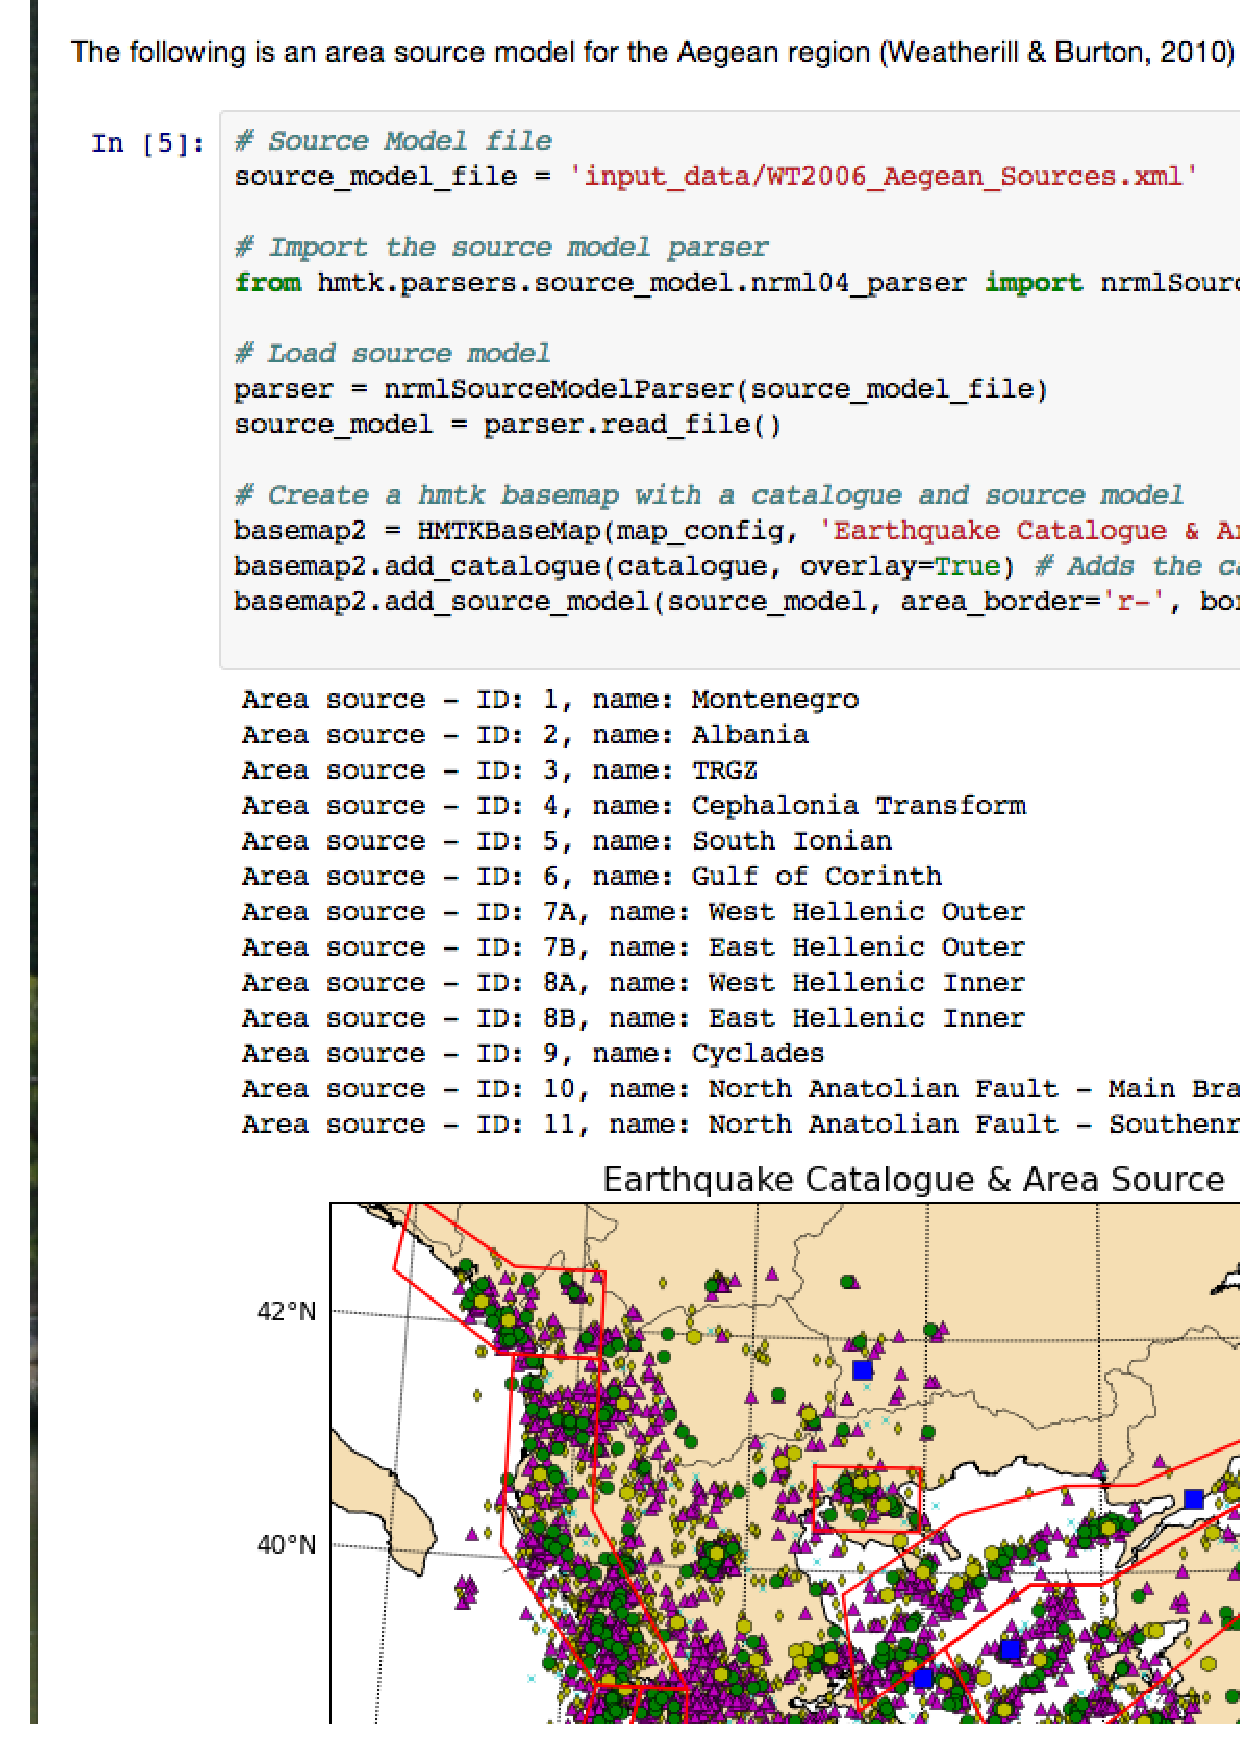
\includegraphics[width=\textwidth]{./figures_v2/hmtk_notebook_screenshot.jpg}
  \caption{Example of the openquake.hmtk embedded in an IPython Notebook}
  \label{fig:notebook}
\end{figure}


\subsection{Visualisation}

In addition to the scientific tools, which will be described in detail in due course, the original version of the openquake.hmtk also included a set of functionalities for visualisation of data and results pertinent to the preparation of seismic hazard input models. While not considered an essential component of the openquake.hmtk, the usage of the plotting functions can facilitate model development. Particular visualisation functions shall be referred to where relevant for the particular tool or data set. 

The current version of the HMTK includes most of the original visualisation tools. However, the tools for map creation have been depracated, and replaced by a set of mapping functions in the \href{https://github.com/GEMScienceTools/oq-mbtk/tree/master/openquake}{OpenQuake Model Building Toolkit (MBTK)}. The tools now use \href{https://www.generic-mapping-tools.org}{Generic Mapping Tools (GMT)}, and so were moved outside of the HMTK library as to not add GMT as a dependency of the OpenQuake Engine. However, the mapping functions are still described in this tutorial in order to provide users with a replacement to the depracated functions. 

\subsubsection{Mapping tools: additional setup}
Within the plotting tools is a set of methods to create maps of geospatial data; these tools are housed in the MBTK. Use of the mapping tools requires the following additional package installations:\\

\begin{enumerate}
	\item \href{https://www.generic-mapping-tools.org/download/}{GMT} version 6.0 or later.
	\item \href{https://github.com/GEMScienceTools/oq-mbtk/tree/master/openquake}{MBTK}\\
\end{enumerate}

The functions of \cprotect{\href{https://github.com/GEMScienceTools/oq-mbtk/tree/master/openquake/plt}}{\verb=openquake.plt.mapping=} can also be used independently of the MBTK (NB: the descriptions herein assume that mapping functions are called through the MBTK). 

\subsubsection{Map Creation}
An IPython Notebook demonstrating how to use the mapping methods can be found \href{https://github.com/GEMScienceTools/oq-mbtk/tree/master/openquake/plt/demo}{in the MBTK}. The basic functionalities are described herein.

To set-up a simple basemap it is necessary to define the configuration of the plot (such as spatial limit and coastline resolution). This is done as follows:

\begin{python}[frame=single]
In [1]: from openquake.plt.mapping import HMTKBaseMap

In [2]: map_config = {"min_lon": 18.0,
                      "max_lon": 32.0,
                       "min_lat": 33.0,
                       "max_lat": 43.0,
		       "title": "Title of Map"}

In [3]: basemap1 = HMTKBaseMap(map_config)
\end{python}

\verb=HMTKBaseMap= is instantiated with a dictionary of configuration parameters: minimum longitude (\verb=min_lon=), maximum longitude (\verb=max_lon=), minimum latitude (\verb=min_lat=), maximum latitude (\verb=max_lat=). The map title (\verb=title=) can also be specified.

A few other configurations can be passed to \verb=HMTKBaseMap= via keyword parameters during the map instantiation:

\begin{itemize}
	\item \verb=projection=: String beginning with '-J' that indicates the map projection, and optionally central meridian and scaling, following the GMT syntax (\href{http://gmt.soest.hawaii.edu/doc/latest/gmt.html\#j-full}{GMT Map Projections}). The default `-JM15c' is a Mercator projection 15 cm wide.
\item \verb=lat_lon_spacing=: Indicates the spacing of latitude and longitude tickmarks. The default is 2 degrees.
\item \verb=output_folder=: Denotes the output directory for the final map and associated files (if saved, see \verb=.savemap=) relative to the local path. The \verb=output_folder= is immeidately created by \verb=HMTKBaseMap=, and used for all temporary files created during the mapping process. The default is \textit{gmt}. 
\item \verb=overwrite=: If True, gives permission to overwrite all existing files in the specified \verb=output_folder=.\\
\end{itemize}

\noindent The class \verb=HMTKBaseMap= contains a set of methods for mapping catalogue data or simplified source models:\\

\noindent \verb;.add_catalogue(cat, scale=0.05, cpt_file=`tmp.cpt', color_field=`depth',;\\
		\verb;logscale=True);\\

\noindent This function will overlay an earthquake catalogue onto the basemap. The input value \verb=cat= is the earthquake catalogue as an instance of the class \\\verb=openquake.hmtk.seismicity.catalogue.Catalogue= (see the next section for details). The catalogue is the only mandatory parameter, but the user can also specify the following optional parameters:\\

\begin{itemize}
	\item \verb=scale=: a scaling coefficient that sets the symbol size per magnitude $m$. Size follows the equation ${\verb=scale=}*10^{(-1.5+m*0.3)}$, where m is magnitude. See GMT documentation.
	\item \verb=cpt_file=: name of an existing color pallet to color earthquake markers. If not specified, the default "tmp.cpt" is generated based on the catalogue \verb=color_field=
	\item \verb=color_field=: the parameter used to color the earthquake markers. The given field must correspond to the catalogue header. If not specified, the markers are colored by depth.
	\item \verb=logscale=: if `True', generates the color pallet according to a log scale. `False' uses a linear color scale. Default is `True'. Ignored if \verb=cpt_file= is specified.\\
\end{itemize}


\begin{figure}[htb]
  \centering
      \includegraphics[width=\textwidth]{./figures_v2/catalogue.jpg}
      %\includegraphics[trim=20mm 14mm 1mm 1mm, clip, width=\textwidth]{./figures_v2/catalogue.jpg}
  \caption{Example visualisation of an Earthquake Catalogue}
  \label{fig:eqcat_simple}
\end{figure}


\noindent \verb;.add_source_model(model);\\

\noindent This method adds a source model to the basemap. The input value \verb=model= is an instance of the class \verb=openquake.hazardlib.nrml.SourceModel= (see section \textbf{TODO -> this is replacing the mtk source classes}). An example of a source model plot is shown in \ref{fig:source_model_map}.

NB: At present, only the following source typologies can be plotted automatically:

\begin{itemize}
\item Point sources
\item Simple faults
\item Complex faults
\item Area sources\\
\end{itemize}

Non-parametric sources and multi-point sources will be added soon.\\
 
\begin{figure}[htb]
  \centering
      \includegraphics[width=\textwidth]{./figures_v2/PNGSourceModel.jpg}
	\caption{Example visualisation of a source model for Papua New Guinea \textcite{ghasemi2016} with area sources (blue) and a complex fault.}
  \label{fig:source_model_map}
\end{figure}


\noindent \verb;.add_colour_scaled_points(longitude, latitude, data, label=`', shape=`-Ss', ;\\
\verb;                                    size=0.3, logscale=False);\\

\noindent This method overlays a set of data points with colour scaled according to the \verb=data= values. Three data arrays are required: one each with the \verb=longitude= and \verb=latitude= coordinates of the data points, and \verb=data=, a set of scalar values (e.g. magnitude or depth, if plotting an earthquake catalogue) associated with those points. In addition to these, the method takes four optional keyword parameters:\\
\begin{itemize}
\item \verb=label=: a string used to label the color scale; corresponds to \verb=data=
\item \verb=shape=: a string indicating the shape of the data markers, using GMT syntax starting with `-S' (see \href{https://docs.generic-mapping-tools.org/latest/psxy.html\#s}{GMT psxy markers}. The default, `-Ss' is squares.
\item \verb=size=: the size in cm of the plotted markers (see \href{https://docs.generic-mapping-tools.org/latest/psxy.html\#s}{GMT psxy markers}). Default is 0.3 cm.
\item \verb=logscale=: if True, use a logscale to create the colorbar. Default is False.\\
\end{itemize}

\begin{figure}[htb]
  \centering
      \includegraphics[width=\textwidth]{./figures_v2/colorscaled.jpg}
	\caption{Example of a seismicity catalogue with color scaled by magnitude.}
  \label{fig:cat_color_scaled}
\end{figure}


\noindent \verb;.add_size_scaled_points(longitude, latitude, data, shape=`-Ss',;\\
\verb;                       logplot=False, color=`blue', smin=0.01, coeff=1.0, ;\\
\verb;                       sscale=2.0, label=`', legend=True);\\

\noindent This method overlays a set of data points with size scaled according to the \verb=data= values. Three data arrays are required: one each with the \verb=longitude= and \verb=latitude= coordinates of points to be plotted, and \verb=data=, a set of scalar values associated with those points. In addition to these, the method takes eight optional keyword parameters:\\

\begin{itemize}
\item \verb=shape=: a string indicating the shape of the data markers, using GMT syntax starting with `-S' (see \href{https://docs.generic-mapping-tools.org/latest/psxy.html\#s}{GMT psxy markers}. The default, `-Ss' is squares.
\item \verb=logplot=: if True, use a logscale to create the marker sizes. Default is False.
\item \verb=color=: a string that indicates the marker color (see \href{https://docs.generic-mapping-tools.org/latest/psxy.html\#w}{GMT psxy markers}. Default is `blue'.
\item \verb=smin=: size of the smallest symbol in cm. Marker size is computed as\\ ${\verb=smin=}+{\verb=coeff=}\times {\verb=data=}^{\verb=sscale=}$. Default is 0.01 cm.
\item \verb=coeff=: used with \verb=sscale= and \verb=smin= to set the marker sizes. Default is 1.0.
\item \verb=sscale=: used with \verb=coeff= and \verb=smin= to set the marker sizes. Default is 2.0.
\item \verb=label=: a string that corresponds to the \verb=data= array
\item \verb=legend=: if True, adds a legend to the plot. Default is True. \\
\end{itemize}

\begin{figure}[htb]
  \centering
      \includegraphics[width=\textwidth]{./figures_v2/sizescaled.jpg}
	\caption{Example of a seismicity catalogue with size scaled by magnitude.}
  \label{fig:source_model_map}
\end{figure}

\noindent \verb;.add_focal_mechanism(filename, mech_format);\\

\noindent This method overlays focal mechanisms. The string \verb=filename= indicates a file containing focal mechanism data. \verb=mech_format= is a string contained by quotations used to indicate the data format used by \verb=filename=, allowing two options---focal mechanism (`FM') and seismic moment tensor (`MT')---both using the Harvard CMT convention, as described by \href{https://docs.generic-mapping-tools.org/latest/supplements/seis/psmeca.html?highlight=psmeca\#s}{GMT psmeca}.\\

\noindent \verb;.savemap(filename=None, save_script=False, verb=False);\\

An instance of \verb=HMTKBaseMap= is not automatically saved. In order to do so, the method \verb=.savemap()= must be called, finalizing and executing the GMT script. The method can take the following three keyword arguments:\\

\begin{itemize}
\item \verb=filename=: a string used to name the map, which includes a suffix (limited to `.pdf', `.png', and `.jpg') indicating the desired file type. If not specified, the map is saved as $map.pdf$ in the directory \verb=output_folder= that was assigned during the \verb=HMTKBaseMap= instantiatation.
\item \verb=save_script=: if True, the GMT commands are saved to a shell script, and this with all files needed to create the map are saved in \verb=output_folder=. If False (the default), all the temporary files are erased and only the map is saved.
\item \verb=verb= (verbose): if True, GMT commands are printed as they are executed.\\
\end{itemize}

The \verb=save_script= option gives the user more flexibility to modify the plot settings than are available through the methods, while providing the structure of the GMT script as a starting point. NB: Take care not to overwrite scripts that have been customized by rerunning the mapping code! \\

The \verb=.savemap()= method is used as follows (continuing from the above Python lines):\\

\begin{python}[frame=single]
In [4]: finame = 'map_demo.pdf'

In [5]: basemap1.savemap(filename=finame, save_script=True)
\end{python}

